\documentclass[a4paper,5pt]{amsbook}
%%%%%%%%%%%%%%%%%%%%%%%%%%%%%%%%%%%%%%%%%%%%%%%%%%%%%%%%%%%%%%%%%%%%%

\usepackage{booktabs}
\usepackage{graphicx}
% \usepackage[]{float}
\usepackage{amssymb}
% \usepackage{amsfonts}
% \usepackage[]{amsmath}
% \usepackage[]{epsfig}
% \usepackage[brazil]{babel}
% \usepackage[utf8]{inputenc}
% \usepackage{verbatim}
%\usepackage[]{pstricks}
%\usepackage[notcite,notref]{showkeys}
\usepackage{subcaption}

%%%%%%%%%%%%%%%%%%%%%%%%%%%%%%%%%%%%%%%%%%%%%%%%%%%%%%%%%%%%%%

\newcommand{\sen}{\,\mbox{sen}\,}
\newcommand{\tg}{\,\mbox{tg}\,}
\newcommand{\cosec}{\,\mbox{cosec}\,}
\newcommand{\cotg}{\,\mbox{cotg}\,}
\newcommand{\ds}{\displaystyle}

%%%%%%%%%%%%%%%%%%%%%%%%%%%%%%%%%%%%%%%%%%%%%%%%%%%%%%%%%%%%%%%%%%%%%%%%

\setlength{\textwidth}{16cm} \setlength{\topmargin}{-1cm}
\setlength{\textheight}{25cm}
\setlength{\leftmargin}{1cm} \setlength{\rightmargin}{1cm}
\setlength{\oddsidemargin}{0cm}\setlength{\evensidemargin}{0cm}

%%%%%%%%%%%%%%%%%%%%%%%%%%%%%%%%%%%%%%%%%%%%%%%%%%%%%%%%%%%%%%%%%%%%%%%%

% \renewcommand{\baselinestretch}{1.6}
% \renewcommand{\thefootnote}{\fnsymbol{footnote}}
% \renewcommand{\theequation}{\thesection.\arabic{equation}}
% \setlength{\voffset}{-50pt}
% \numberwithin{equation}{chapter}

%%%%%%%%%%%%%%%%%%%%%%%%%%%%%%%%%%%%%%%%%%%%%%%%%%%%%%%%%%%%%%%%%%%%%%%

\begin{document}
\thispagestyle{empty}
\hspace{-0.6cm}
\begin{minipage}[p]{0.14\linewidth}
	
\includegraphics[scale=0.24]{ufgd.png}
\end{minipage}
\begin{minipage}[p]{0.7\linewidth}
\begin{tabular}{c}
\toprule{}
{{\bf UNIVERSIDADE FEDERAL DA GRANDE DOURADOS}}\\
{{\bf Prof.\ Adriano Barbosa}}\\

{{\bf C\'alculo 2 --- Avalia\c{c}\~ao P1}}\\

\midrule{}
Eng.\ Mec\^anica\hspace{5cm}3 de Fevereiro de 2017 \\
\bottomrule{}
\end{tabular}
\vspace{-0.45cm}
%
\end{minipage}
\begin{minipage}[p]{0.15\linewidth}
\begin{flushright}
\def\arraystretch{1.2}
\begin{tabular}{|c|c|}  % chktex 44
\hline\hline  % chktex 44
1 & \hspace{1.2cm} \\
\hline  % chktex 44
2& \\
\hline  % chktex 44
3& \\
\hline  % chktex 44
4&  \\
\hline  % chktex 44
5&  \\
\hline  % chktex 44
{\small Total}&  \\
\hline\hline  % chktex 44
\end{tabular}
\end{flushright}
\end{minipage}

%------------------------
\vspace{0.5cm}
{\bf Aluno(a):}\dotfill{}  % chktex 36
%----------------------------

\vspace{0.2cm}
%%%%%%%%%%%%%%%%%%%%%%%%%%%%%%%%   formulario  inicio  %%%%%%%%%%%%%%%%%%%%%%%%%%%%%%%%
\begin{enumerate}
	\vspace{0.5cm}

	\item Calcule a integral definida $\ds\int_1^2 \frac{x}{{(1+x)}^2}\ dx$.
	\vspace{0.5cm}

	\item Dados os polin\^omios $p(x) = x^2 + 8x - 3$ e $q(x) = x^3 + x^2$:
		\begin{enumerate}
				\vspace{0.2cm}
			\item Fatore o polin\^omio $q(x)$.
				\vspace{0.1cm}
			\item Escreva $\ds\frac{p(x)}{q(x)}$ como soma de fra\c{c}\~oes parciais.
			\item Calcule a integral $\ds\int \frac{p(x)}{q(x)}\ dx$.
		\end{enumerate}
	\vspace{0.5cm}

	\item Calcule a integral indefinida $\ds\int x \sen{(x)} \cos{(x)}\ dx$.
	\vspace{0.5cm}

	\item Calcule a \'area da regi\~ao delimitada pelo gr\'afico da curva $x^2 + y^2
		= 4$, as retas $x = -1$, $x = 1$ e o eixo $x$.
		\begin{figure}[h]
			\centering
			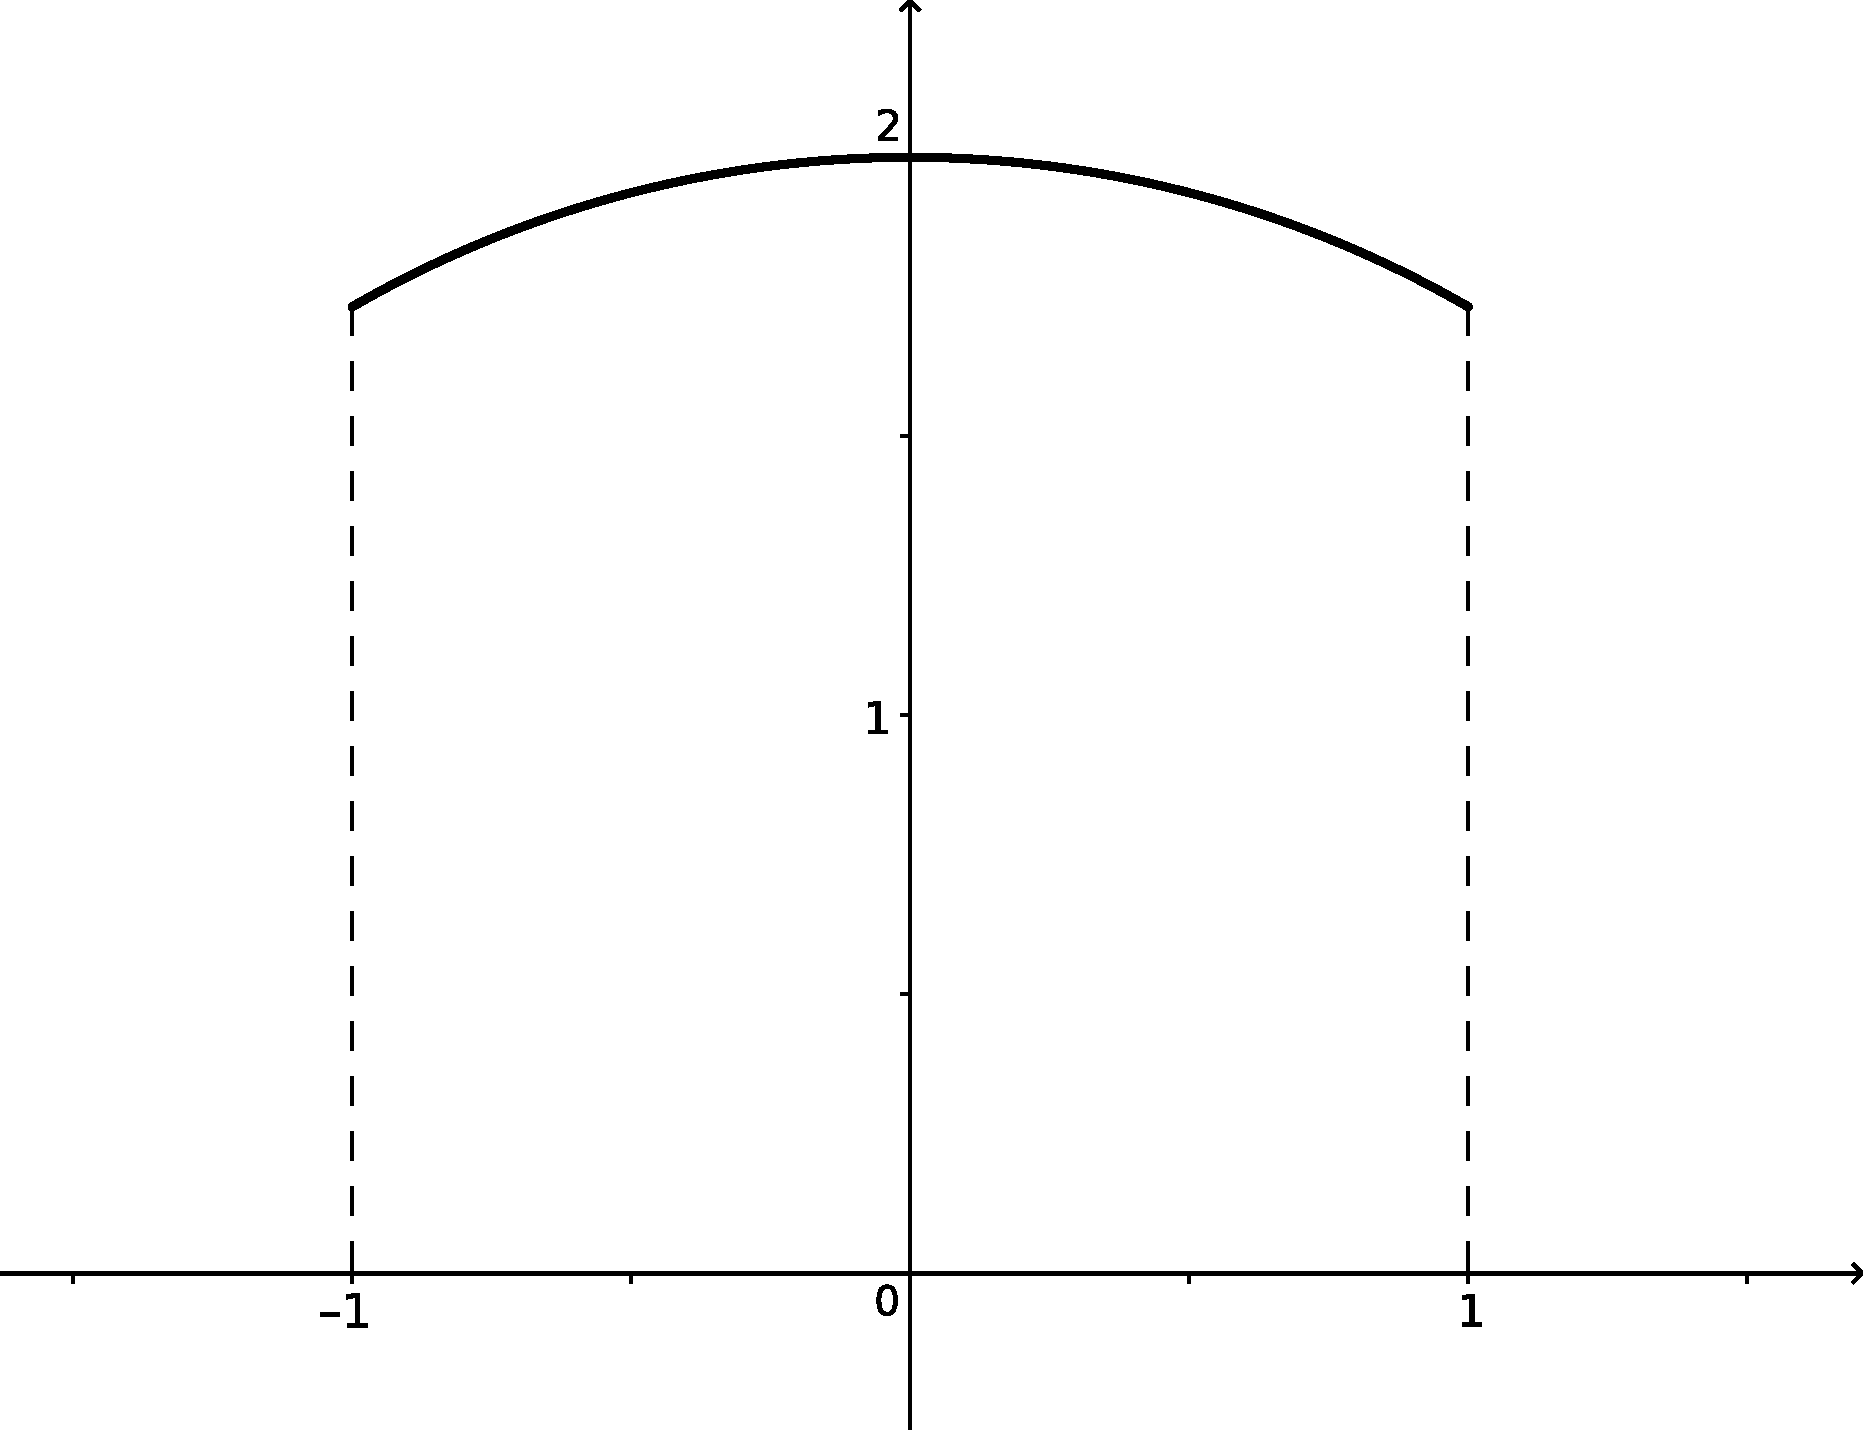
\includegraphics[width=0.3\textwidth]{grafico.pdf}
		\end{figure}

	\vspace{0.5cm}

	\item Calcule a integral impr\'opria $\ds\int_0^{\pi}\,\text{tg}\,(x)\ dx$.
	\vspace{0.5cm}
	\vspace{0.5cm}

\end{enumerate}

F\'ormulas \'uteis:

\[\begin{array}{cccc}
	\vspace{0.5cm}
	\cosec(x) = \displaystyle\frac{1}{\sen(x)} & \sec(x) = \displaystyle\frac{1}{\cos(x)} & \cotg(x) = \displaystyle\frac{\cos(x)}{\sen(x)} & \ds\tg(x) = \frac{\sen(x)}{\cos(x)}\\
	\vspace{0.5cm}
	\sen^2(x) + \cos^2(x) = 1 & \tg^2(x) + 1 = \sec^2(x) & 1 + \cotg^2(x) = \cosec^2(x) & \\
	\vspace{0.5cm}
	\sen^2(x) = \displaystyle\frac{1 - \cos(2x)}{2} & \cos^2(x) = \displaystyle\frac{1 + \cos(2x)}{2} & & 
\end{array}\]

\begin{flushright}
	\textit{Boa Prova!}
\end{flushright}

\end{document}
